\documentclass[11pt]{article}
\usepackage{enumerate}
\usepackage{tikz}
\usepackage{fullpage}
\usepackage{fancyhdr}
\usepackage{graphicx}

\usepackage{amsmath, amsfonts, amsthm, amssymb}
\setlength{\parindent}{0pt}
\setlength{\parskip}{5pt plus 1pt}
\pagestyle{empty}

\def\indented#1{\list{}{}\item[]}
\let\indented=\endlist

\newcounter{questionCounter}
\newcounter{partCounter}[questionCounter]
\newenvironment{question}[2][\arabic{questionCounter}]{%
    \setcounter{partCounter}{0}%
    \vspace{.25in} \hrule \vspace{0.5em}%
        \noindent{\bf #2}%
    \vspace{0.8em} \hrule \vspace{.10in}%
    \addtocounter{questionCounter}{1}%
}{}
\renewenvironment{part}[1][\alph{partCounter}]{%
    \addtocounter{partCounter}{1}%
    \vspace{.10in}%
    \begin{indented}%
       {\bf (#1)} %
}{\end{indented}}

%%%%%%%%%%%%%%%%% Identifying Information %%%%%%%%%%%%%%%%%
%% This is here, so that you can make your homework look %%
%% pretty when you compile it.                           %%
%%     DO NOT PUT YOUR NAME ANYWHERE ELSE!!!!            %%
%%%%%%%%%%%%%%%%%%%%%%%%%%%%%%%%%%%%%%%%%%%%%%%%%%%%%%%%%%%
\newcommand{\myname}{Michael Choquette, Rokhini Prabhu}
\newcommand{\myandrew}{mchoquet, rokhinip}
\newcommand{\myhwname}{Assignment 2}
%%%%%%%%%%%%%%%%%%%%%%%%%%%%%%%%%%%%%%%%%%%%%%%%%%%%%%%%%%%

\begin{document}
\thispagestyle{plain}

\begin{center}
{\Large \myhwname} \\
\myname \\
\myandrew \\
\today
\end{center}

\newcommand{\code}[1]{\texttt{#1}}
\begin{question}{Writeup}
\end{question}
\begin{question}{Lazy Code Motion}

After the Anticipated expressions pass: Each block is annotated with 
the in and out values of \texttt{anticipated}
\begin{center}
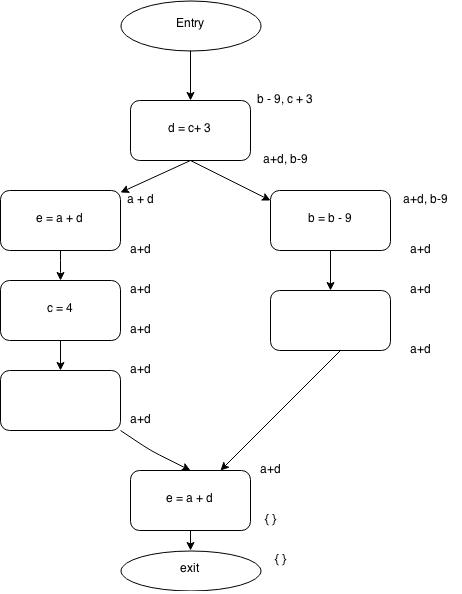
\includegraphics[scale=0.5]{cfg1.jpg}
\end{center}

After the Early Placement pass: Each block is annotated with the values 
of \texttt{earliest} for that block.
\begin{center}
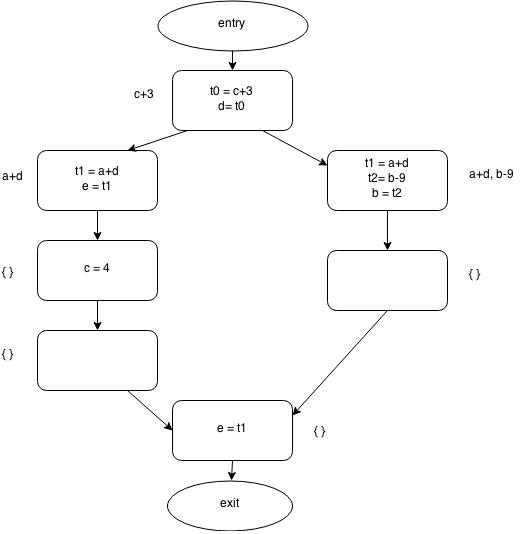
\includegraphics[scale=0.5]{cfg2.jpg}
\end{center}

After Lazy Code Motion and cleanup passes:
\begin{center}
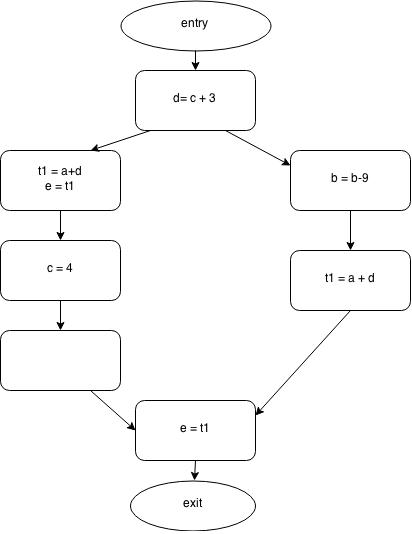
\includegraphics[scale=0.5]{cfg3.jpg}
\end{center}
\end{question}
\begin{question}{Loop Invariant Code Motion}
\end{question}
\end{document}
